% Generated by Sphinx.
\documentclass[a4paper,10pt,english]{manual}
\usepackage[utf8]{inputenc}
\usepackage[T1]{fontenc}
\usepackage{babel}
\usepackage{times}
\usepackage[Bjarne]{fncychap}
\usepackage{longtable}
\usepackage{sphinx}


\title{BIP - Bayesian Inference with Python Documentation}
\date{March 01, 2010}
\release{0.3}
\author{Flávio Codeço Coelho}
\newcommand{\sphinxlogo}{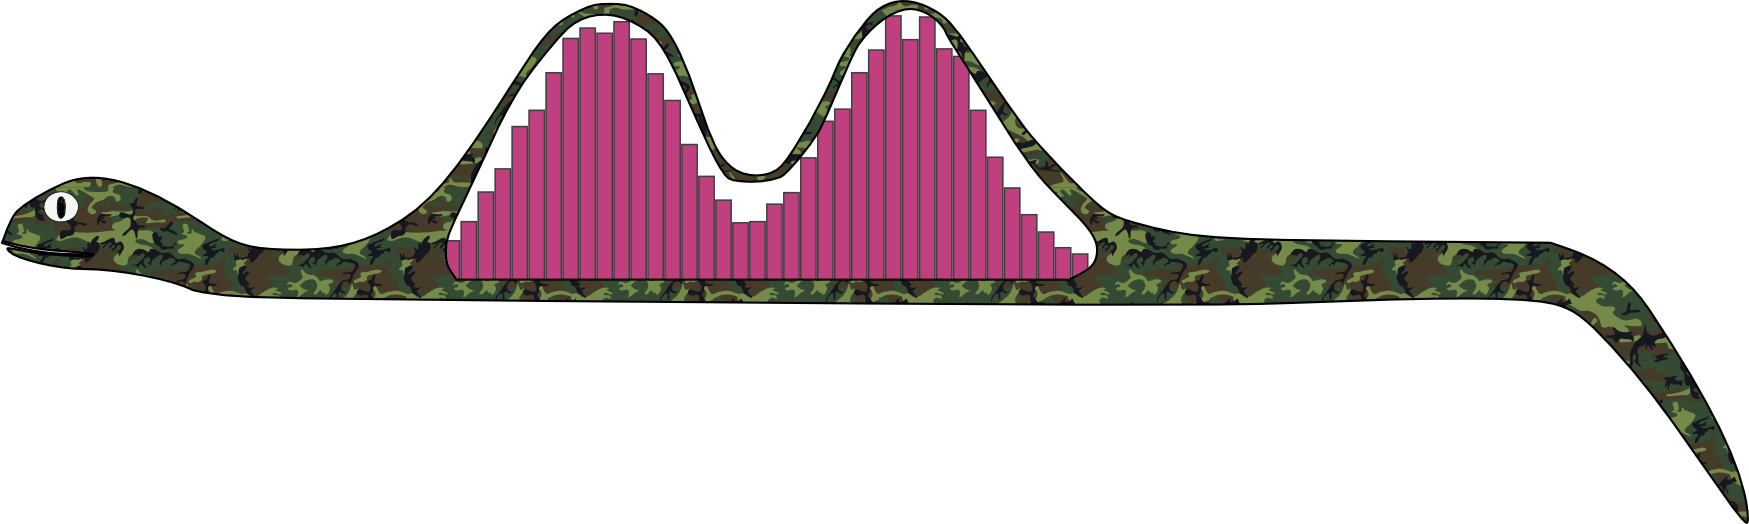
\includegraphics{BIP_large.png}\par}
\renewcommand{\releasename}{Release}
\makeindex
\makemodindex

\makeatletter
\def\PYG@reset{\let\PYG@it=\relax \let\PYG@bf=\relax%
    \let\PYG@ul=\relax \let\PYG@tc=\relax%
    \let\PYG@bc=\relax \let\PYG@ff=\relax}
\def\PYG@tok#1{\csname PYG@tok@#1\endcsname}
\def\PYG@toks#1+{\ifx\relax#1\empty\else%
    \PYG@tok{#1}\expandafter\PYG@toks\fi}
\def\PYG@do#1{\PYG@bc{\PYG@tc{\PYG@ul{%
    \PYG@it{\PYG@bf{\PYG@ff{#1}}}}}}}
\def\PYG#1#2{\PYG@reset\PYG@toks#1+\relax+\PYG@do{#2}}

\def\PYG@tok@gd{\def\PYG@tc##1{\textcolor[rgb]{0.63,0.00,0.00}{##1}}}
\def\PYG@tok@gu{\let\PYG@bf=\textbf\def\PYG@tc##1{\textcolor[rgb]{0.50,0.00,0.50}{##1}}}
\def\PYG@tok@gt{\def\PYG@tc##1{\textcolor[rgb]{0.00,0.25,0.82}{##1}}}
\def\PYG@tok@gs{\let\PYG@bf=\textbf}
\def\PYG@tok@gr{\def\PYG@tc##1{\textcolor[rgb]{1.00,0.00,0.00}{##1}}}
\def\PYG@tok@cm{\let\PYG@it=\textit\def\PYG@tc##1{\textcolor[rgb]{0.25,0.50,0.56}{##1}}}
\def\PYG@tok@vg{\def\PYG@tc##1{\textcolor[rgb]{0.73,0.38,0.84}{##1}}}
\def\PYG@tok@m{\def\PYG@tc##1{\textcolor[rgb]{0.13,0.50,0.31}{##1}}}
\def\PYG@tok@mh{\def\PYG@tc##1{\textcolor[rgb]{0.13,0.50,0.31}{##1}}}
\def\PYG@tok@cs{\def\PYG@tc##1{\textcolor[rgb]{0.25,0.50,0.56}{##1}}\def\PYG@bc##1{\colorbox[rgb]{1.00,0.94,0.94}{##1}}}
\def\PYG@tok@ge{\let\PYG@it=\textit}
\def\PYG@tok@vc{\def\PYG@tc##1{\textcolor[rgb]{0.73,0.38,0.84}{##1}}}
\def\PYG@tok@il{\def\PYG@tc##1{\textcolor[rgb]{0.13,0.50,0.31}{##1}}}
\def\PYG@tok@go{\def\PYG@tc##1{\textcolor[rgb]{0.19,0.19,0.19}{##1}}}
\def\PYG@tok@cp{\def\PYG@tc##1{\textcolor[rgb]{0.00,0.44,0.13}{##1}}}
\def\PYG@tok@gi{\def\PYG@tc##1{\textcolor[rgb]{0.00,0.63,0.00}{##1}}}
\def\PYG@tok@gh{\let\PYG@bf=\textbf\def\PYG@tc##1{\textcolor[rgb]{0.00,0.00,0.50}{##1}}}
\def\PYG@tok@ni{\let\PYG@bf=\textbf\def\PYG@tc##1{\textcolor[rgb]{0.84,0.33,0.22}{##1}}}
\def\PYG@tok@nl{\let\PYG@bf=\textbf\def\PYG@tc##1{\textcolor[rgb]{0.00,0.13,0.44}{##1}}}
\def\PYG@tok@nn{\let\PYG@bf=\textbf\def\PYG@tc##1{\textcolor[rgb]{0.05,0.52,0.71}{##1}}}
\def\PYG@tok@no{\def\PYG@tc##1{\textcolor[rgb]{0.38,0.68,0.84}{##1}}}
\def\PYG@tok@na{\def\PYG@tc##1{\textcolor[rgb]{0.25,0.44,0.63}{##1}}}
\def\PYG@tok@nb{\def\PYG@tc##1{\textcolor[rgb]{0.00,0.44,0.13}{##1}}}
\def\PYG@tok@nc{\let\PYG@bf=\textbf\def\PYG@tc##1{\textcolor[rgb]{0.05,0.52,0.71}{##1}}}
\def\PYG@tok@nd{\let\PYG@bf=\textbf\def\PYG@tc##1{\textcolor[rgb]{0.33,0.33,0.33}{##1}}}
\def\PYG@tok@ne{\def\PYG@tc##1{\textcolor[rgb]{0.00,0.44,0.13}{##1}}}
\def\PYG@tok@nf{\def\PYG@tc##1{\textcolor[rgb]{0.02,0.16,0.49}{##1}}}
\def\PYG@tok@si{\let\PYG@it=\textit\def\PYG@tc##1{\textcolor[rgb]{0.44,0.63,0.82}{##1}}}
\def\PYG@tok@s2{\def\PYG@tc##1{\textcolor[rgb]{0.25,0.44,0.63}{##1}}}
\def\PYG@tok@vi{\def\PYG@tc##1{\textcolor[rgb]{0.73,0.38,0.84}{##1}}}
\def\PYG@tok@nt{\let\PYG@bf=\textbf\def\PYG@tc##1{\textcolor[rgb]{0.02,0.16,0.45}{##1}}}
\def\PYG@tok@nv{\def\PYG@tc##1{\textcolor[rgb]{0.73,0.38,0.84}{##1}}}
\def\PYG@tok@s1{\def\PYG@tc##1{\textcolor[rgb]{0.25,0.44,0.63}{##1}}}
\def\PYG@tok@gp{\let\PYG@bf=\textbf\def\PYG@tc##1{\textcolor[rgb]{0.78,0.36,0.04}{##1}}}
\def\PYG@tok@sh{\def\PYG@tc##1{\textcolor[rgb]{0.25,0.44,0.63}{##1}}}
\def\PYG@tok@ow{\let\PYG@bf=\textbf\def\PYG@tc##1{\textcolor[rgb]{0.00,0.44,0.13}{##1}}}
\def\PYG@tok@sx{\def\PYG@tc##1{\textcolor[rgb]{0.78,0.36,0.04}{##1}}}
\def\PYG@tok@bp{\def\PYG@tc##1{\textcolor[rgb]{0.00,0.44,0.13}{##1}}}
\def\PYG@tok@c1{\let\PYG@it=\textit\def\PYG@tc##1{\textcolor[rgb]{0.25,0.50,0.56}{##1}}}
\def\PYG@tok@kc{\let\PYG@bf=\textbf\def\PYG@tc##1{\textcolor[rgb]{0.00,0.44,0.13}{##1}}}
\def\PYG@tok@c{\let\PYG@it=\textit\def\PYG@tc##1{\textcolor[rgb]{0.25,0.50,0.56}{##1}}}
\def\PYG@tok@mf{\def\PYG@tc##1{\textcolor[rgb]{0.13,0.50,0.31}{##1}}}
\def\PYG@tok@err{\def\PYG@bc##1{\fcolorbox[rgb]{1.00,0.00,0.00}{1,1,1}{##1}}}
\def\PYG@tok@kd{\let\PYG@bf=\textbf\def\PYG@tc##1{\textcolor[rgb]{0.00,0.44,0.13}{##1}}}
\def\PYG@tok@ss{\def\PYG@tc##1{\textcolor[rgb]{0.32,0.47,0.09}{##1}}}
\def\PYG@tok@sr{\def\PYG@tc##1{\textcolor[rgb]{0.14,0.33,0.53}{##1}}}
\def\PYG@tok@mo{\def\PYG@tc##1{\textcolor[rgb]{0.13,0.50,0.31}{##1}}}
\def\PYG@tok@mi{\def\PYG@tc##1{\textcolor[rgb]{0.13,0.50,0.31}{##1}}}
\def\PYG@tok@kn{\let\PYG@bf=\textbf\def\PYG@tc##1{\textcolor[rgb]{0.00,0.44,0.13}{##1}}}
\def\PYG@tok@o{\def\PYG@tc##1{\textcolor[rgb]{0.40,0.40,0.40}{##1}}}
\def\PYG@tok@kr{\let\PYG@bf=\textbf\def\PYG@tc##1{\textcolor[rgb]{0.00,0.44,0.13}{##1}}}
\def\PYG@tok@s{\def\PYG@tc##1{\textcolor[rgb]{0.25,0.44,0.63}{##1}}}
\def\PYG@tok@kp{\def\PYG@tc##1{\textcolor[rgb]{0.00,0.44,0.13}{##1}}}
\def\PYG@tok@w{\def\PYG@tc##1{\textcolor[rgb]{0.73,0.73,0.73}{##1}}}
\def\PYG@tok@kt{\def\PYG@tc##1{\textcolor[rgb]{0.56,0.13,0.00}{##1}}}
\def\PYG@tok@sc{\def\PYG@tc##1{\textcolor[rgb]{0.25,0.44,0.63}{##1}}}
\def\PYG@tok@sb{\def\PYG@tc##1{\textcolor[rgb]{0.25,0.44,0.63}{##1}}}
\def\PYG@tok@k{\let\PYG@bf=\textbf\def\PYG@tc##1{\textcolor[rgb]{0.00,0.44,0.13}{##1}}}
\def\PYG@tok@se{\let\PYG@bf=\textbf\def\PYG@tc##1{\textcolor[rgb]{0.25,0.44,0.63}{##1}}}
\def\PYG@tok@sd{\let\PYG@it=\textit\def\PYG@tc##1{\textcolor[rgb]{0.25,0.44,0.63}{##1}}}

\def\PYGZat{@}
\def\PYGZlb{[}
\def\PYGZrb{]}
\makeatother

\begin{document}

\maketitle
\tableofcontents
\hypertarget{--doc-index}{}


Contents:

\resetcurrentobjects
\hypertarget{--doc-overview}{}

\chapter{Overview}

The Bip Package is a collection of useful classes for basic Bayesian inference. Currently, its main goal is to be a tool for learning and exploration of Bayesian probabilistic calculations.

Currently it also includes subpackages for stochastic simulation tools which are not strictly related to Bayesian inference, but are currently being developed within BIP. One such package is the BIP.SDE which contains a parallelized solver for stochastic differential equations, an implementation of the Gillespie direct algorithm.

The Subpackage Bayes also offers a tool for parameter estimation of Deterministic and Stochastic Dynamical Models. This tool will be fully described briefly in a scientific paper currently submitted for publication.

\resetcurrentobjects
\hypertarget{--doc-paramest}{}

\chapter{Parameter Estimation in Dynamic Models}

A growing theme in mathamatical modeling is uncertainty analysis. The Melding Module provides a Bayesian framework to analyze uncertainty in mathematical models. It includes tools that allow modellers to integrate Prior information about the model's parameters and variables into the model, in order to explore the full uncertainty associated with a model.

Once a model is thus parameterized, we can simulate the model, with full uncertainty representation and also fit the model to available data to reduce that uncertaity. Markov chain Monte Carlo algorithms are at the core of the framework, which requires a large number of simulations of the models in order to explore parameter space.


\section{Example Usage}

This first example includes a simple ODE (an epidemic model) model which is fitted against simulated data to which noise is added:

\begin{Verbatim}[commandchars=@\[\]]
@PYG[k+kn][from] @PYG[n+nn][BIP.Bayes.Melding] @PYG[k+kn][import] @PYG[n][FitModel]
@PYG[k+kn][from] @PYG[n+nn][scipy.integrate] @PYG[k+kn][import] @PYG[n][odeint]
@PYG[k+kn][import] @PYG[n+nn][scipy.stats] @PYG[k+kn][as] @PYG[n+nn][st]
@PYG[k+kn][import] @PYG[n+nn][numpy] @PYG[k+kn][as] @PYG[n+nn][np]

@PYG[n][beta] @PYG[o][=] @PYG[l+m+mi][1] @PYG[c][@#Transmission coefficient]
@PYG[n][tau] @PYG[o][=] @PYG[o][.]@PYG[l+m+mi][2] @PYG[c][@#infectious period. FIXED]
@PYG[n][t0] @PYG[o][=] @PYG[l+m+mi][0]
@PYG[n][tf] @PYG[o][=] @PYG[l+m+mi][36]
@PYG[n][y0] @PYG[o][=] @PYG[p][@PYGZlb[]]@PYG[o][.]@PYG[l+m+mi][999]@PYG[p][,]@PYG[l+m+mf][0.001]@PYG[p][,]@PYG[l+m+mf][0.0]@PYG[p][@PYGZrb[]]
@PYG[k][def] @PYG[n+nf][model]@PYG[p][(]@PYG[o][*]@PYG[n][theta]@PYG[p][)]@PYG[p][:]
        @PYG[n][beta] @PYG[o][=] @PYG[n][theta]@PYG[p][@PYGZlb[]]@PYG[l+m+mi][0]@PYG[p][@PYGZrb[]]
        @PYG[k][def] @PYG[n+nf][sir]@PYG[p][(]@PYG[n][y]@PYG[p][,]@PYG[n][t]@PYG[p][)]@PYG[p][:]
                @PYG[l+s+sd]['''ODE model''']
                @PYG[n][S]@PYG[p][,]@PYG[n][I]@PYG[p][,]@PYG[n][R] @PYG[o][=] @PYG[n][y]
                @PYG[k][return]  @PYG[p][@PYGZlb[]]@PYG[o][-]@PYG[n][beta]@PYG[o][*]@PYG[n][I]@PYG[o][*]@PYG[n][S]@PYG[p][,] @PYG[c][@#dS/dt]
                                @PYG[n][beta]@PYG[o][*]@PYG[n][I]@PYG[o][*]@PYG[n][S] @PYG[o][-] @PYG[n][tau]@PYG[o][*]@PYG[n][I]@PYG[p][,] @PYG[c][@#dI/dt]
                                @PYG[n][tau]@PYG[o][*]@PYG[n][I]@PYG[p][@PYGZrb[]] @PYG[c][@#dR/dt]
        @PYG[n][y] @PYG[o][=] @PYG[n][odeint]@PYG[p][(]@PYG[n][sir]@PYG[p][,]@PYG[n][inits]@PYG[p][,]@PYG[n][np]@PYG[o][.]@PYG[n][arange]@PYG[p][(]@PYG[n][t0]@PYG[p][,]@PYG[n][tf]@PYG[p][,]@PYG[l+m+mi][1]@PYG[p][)]@PYG[p][)]@PYG[c][@#np.arange(t0,tf,step))]
        @PYG[k][return] @PYG[n][y]

@PYG[n][F] @PYG[o][=] @PYG[n][FitModel]@PYG[p][(]@PYG[l+m+mi][3000]@PYG[p][,]@PYG[l+m+mi][1000]@PYG[p][,]@PYG[n][model]@PYG[p][,]@PYG[l+m+mi][1]@PYG[p][,]@PYG[l+m+mi][3]@PYG[p][,]@PYG[n][y0]@PYG[p][,]@PYG[n][tf]@PYG[p][,]@PYG[p][@PYGZlb[]]@PYG[l+s][']@PYG[l+s][beta]@PYG[l+s][']@PYG[p][@PYGZrb[]]@PYG[p][,]@PYG[p][@PYGZlb[]]@PYG[l+s][']@PYG[l+s][S]@PYG[l+s][']@PYG[p][,]@PYG[l+s][']@PYG[l+s][I]@PYG[l+s][']@PYG[p][,]@PYG[l+s][']@PYG[l+s][R]@PYG[l+s][']@PYG[p][@PYGZrb[]]@PYG[p][,]
                        @PYG[n][wl]@PYG[o][=]@PYG[l+m+mi][36]@PYG[p][,]@PYG[n][nw]@PYG[o][=]@PYG[l+m+mi][1]@PYG[p][,]@PYG[n][verbose]@PYG[o][=]@PYG[n+nb+bp][False]@PYG[p][,]@PYG[n][burnin]@PYG[o][=]@PYG[l+m+mi][1000]@PYG[p][)]
@PYG[n][F]@PYG[o][.]@PYG[n][set@_priors]@PYG[p][(]@PYG[n][tdists]@PYG[o][=]@PYG[p][@PYGZlb[]]@PYG[n][st]@PYG[o][.]@PYG[n][norm]@PYG[p][@PYGZrb[]]@PYG[p][,]@PYG[n][tpars]@PYG[o][=]@PYG[p][@PYGZlb[]]@PYG[p][(]@PYG[l+m+mf][1.1]@PYG[p][,]@PYG[o][.]@PYG[l+m+mi][2]@PYG[p][)]@PYG[p][@PYGZrb[]]@PYG[p][,]@PYG[n][tlims]@PYG[o][=]@PYG[p][@PYGZlb[]]@PYG[p][(]@PYG[l+m+mf][0.5]@PYG[p][,]@PYG[l+m+mf][1.5]@PYG[p][)]@PYG[p][@PYGZrb[]]@PYG[p][,]
        @PYG[n][pdists]@PYG[o][=]@PYG[p][@PYGZlb[]]@PYG[n][st]@PYG[o][.]@PYG[n][uniform]@PYG[p][@PYGZrb[]]@PYG[o][*]@PYG[l+m+mi][3]@PYG[p][,]@PYG[n][ppars]@PYG[o][=]@PYG[p][@PYGZlb[]]@PYG[p][(]@PYG[l+m+mi][0]@PYG[p][,]@PYG[o][.]@PYG[l+m+mi][1]@PYG[p][)]@PYG[p][,]@PYG[p][(]@PYG[l+m+mi][0]@PYG[p][,]@PYG[o][.]@PYG[l+m+mi][1]@PYG[p][)]@PYG[p][,]@PYG[p][(]@PYG[o][.]@PYG[l+m+mi][8]@PYG[p][,]@PYG[o][.]@PYG[l+m+mi][2]@PYG[p][)]@PYG[p][@PYGZrb[]]@PYG[p][,]@PYG[n][plims]@PYG[o][=]@PYG[p][@PYGZlb[]]@PYG[p][(]@PYG[l+m+mi][0]@PYG[p][,]@PYG[l+m+mi][1]@PYG[p][)]@PYG[p][@PYGZrb[]]@PYG[o][*]@PYG[l+m+mi][3]@PYG[p][)]
@PYG[n][d] @PYG[o][=] @PYG[n][model]@PYG[p][(]@PYG[o][*]@PYG[p][@PYGZlb[]]@PYG[l+m+mf][1.0]@PYG[p][@PYGZrb[]]@PYG[p][)] @PYG[c][@#simulate some data]
@PYG[n][noise] @PYG[o][=] @PYG[n][st]@PYG[o][.]@PYG[n][norm]@PYG[p][(]@PYG[l+m+mi][0]@PYG[p][,]@PYG[l+m+mf][0.01]@PYG[p][)]@PYG[o][.]@PYG[n][rvs]@PYG[p][(]@PYG[l+m+mi][36]@PYG[p][)]
@PYG[n][dt] @PYG[o][=] @PYG[p][{]@PYG[l+s][']@PYG[l+s][I]@PYG[l+s][']@PYG[p][:]@PYG[n][d]@PYG[p][@PYGZlb[]]@PYG[p][:]@PYG[p][,]@PYG[l+m+mi][1]@PYG[p][@PYGZrb[]]@PYG[o][+]@PYG[n][noise]@PYG[p][}] @PYG[c][@# add noise]
@PYG[n][F]@PYG[o][.]@PYG[n][run]@PYG[p][(]@PYG[n][dt]@PYG[p][,]@PYG[l+s][']@PYG[l+s][MCMC]@PYG[l+s][']@PYG[p][,]@PYG[n][likvar]@PYG[o][=]@PYG[l+m+mf][1e-2]@PYG[p][,]@PYG[n][pool]@PYG[o][=]@PYG[n+nb+bp][True]@PYG[p][,]@PYG[n][monitor]@PYG[o][=]@PYG[p][@PYGZlb[]]@PYG[l+s][']@PYG[l+s][I]@PYG[l+s][']@PYG[p][@PYGZrb[]]@PYG[p][)]
@PYG[n][F]@PYG[o][.]@PYG[n][plot@_results]@PYG[p][(]@PYG[p][)]
\end{Verbatim}

The code above starts by defining the models parameters and initial conditions, and a function which takes in the parameters runs the model and returns the output.

After that, we Instantiate our fitting Object:

\begin{Verbatim}[commandchars=@\[\]]
@PYG[n][F] @PYG[o][=] @PYG[n][FitModel]@PYG[p][(]@PYG[l+m+mi][3000]@PYG[p][,]@PYG[l+m+mi][1000]@PYG[p][,]@PYG[n][model]@PYG[p][,]@PYG[l+m+mi][1]@PYG[p][,]@PYG[l+m+mi][3]@PYG[p][,]@PYG[n][y0]@PYG[p][,]@PYG[n][tf]@PYG[p][,]@PYG[p][@PYGZlb[]]@PYG[l+s][']@PYG[l+s][beta]@PYG[l+s][']@PYG[p][@PYGZrb[]]@PYG[p][,]@PYG[p][@PYGZlb[]]@PYG[l+s][']@PYG[l+s][S]@PYG[l+s][']@PYG[p][,]@PYG[l+s][']@PYG[l+s][I]@PYG[l+s][']@PYG[p][,]@PYG[l+s][']@PYG[l+s][R]@PYG[l+s][']@PYG[p][@PYGZrb[]]@PYG[p][,]
                        @PYG[n][wl]@PYG[o][=]@PYG[l+m+mi][36]@PYG[p][,]@PYG[n][nw]@PYG[o][=]@PYG[l+m+mi][1]@PYG[p][,]@PYG[n][verbose]@PYG[o][=]@PYG[n+nb+bp][False]@PYG[p][,]@PYG[n][burnin]@PYG[o][=]@PYG[l+m+mi][1000]@PYG[p][)]
\end{Verbatim}

Here we have to pass a few arguments: the first (\code{K=3000}) is the number of samples we will take from the joint prior distribution of the parameters to run the inference. The second one (\code{L=1000}) is the number to retain if the inference method chosen (see below) in the sampling-importance-resampling (SIR) or approximate Bayes (ABC). then we we have the number of parameters to be analyzed (\code{ntheta=1}), the number of output variables (\code{nphi=3}), the initial condition vector(\code{inits=y0}), the list of parameter names (\code{thetanames = {[}'beta'{]}}), the list of variable names (\code{phinames={[}'S','I','R'{]}}), inference window length (\code{wl=36}), number of juxtaposed windows (\code{nw=1}), verbosity flag (\code{verbose=False}) and finally the number of burnin samples (\code{burnin=1000}), which is only needed for if the inference method chosen is \code{MCMC}.

The next line of code also carries a lot of relevant information about the inference: the specification of the prior distributions. By now you must have noticed that not all parameters included in the model need to be included in the analysis. any number of them except for one can be set constant, which is what happens with the parameter \code{tau} in this example:

\begin{Verbatim}[commandchars=@\[\]]
@PYG[n][F]@PYG[o][.]@PYG[n][set@_priors]@PYG[p][(]@PYG[n][tdists]@PYG[o][=]@PYG[p][@PYGZlb[]]@PYG[n][st]@PYG[o][.]@PYG[n][norm]@PYG[p][@PYGZrb[]]@PYG[p][,]@PYG[n][tpars]@PYG[o][=]@PYG[p][@PYGZlb[]]@PYG[p][(]@PYG[l+m+mf][1.1]@PYG[p][,]@PYG[o][.]@PYG[l+m+mi][2]@PYG[p][)]@PYG[p][@PYGZrb[]]@PYG[p][,]@PYG[n][tlims]@PYG[o][=]@PYG[p][@PYGZlb[]]@PYG[p][(]@PYG[l+m+mf][0.5]@PYG[p][,]@PYG[l+m+mf][1.5]@PYG[p][)]@PYG[p][@PYGZrb[]]@PYG[p][,]
        @PYG[n][pdists]@PYG[o][=]@PYG[p][@PYGZlb[]]@PYG[n][st]@PYG[o][.]@PYG[n][uniform]@PYG[p][@PYGZrb[]]@PYG[o][*]@PYG[l+m+mi][3]@PYG[p][,]@PYG[n][ppars]@PYG[o][=]@PYG[p][@PYGZlb[]]@PYG[p][(]@PYG[l+m+mi][0]@PYG[p][,]@PYG[o][.]@PYG[l+m+mi][1]@PYG[p][)]@PYG[p][,]@PYG[p][(]@PYG[l+m+mi][0]@PYG[p][,]@PYG[o][.]@PYG[l+m+mi][1]@PYG[p][)]@PYG[p][,]@PYG[p][(]@PYG[o][.]@PYG[l+m+mi][8]@PYG[p][,]@PYG[o][.]@PYG[l+m+mi][2]@PYG[p][)]@PYG[p][@PYGZrb[]]@PYG[p][,]@PYG[n][plims]@PYG[o][=]@PYG[p][@PYGZlb[]]@PYG[p][(]@PYG[l+m+mi][0]@PYG[p][,]@PYG[l+m+mi][1]@PYG[p][)]@PYG[p][@PYGZrb[]]@PYG[o][*]@PYG[l+m+mi][3]@PYG[p][)]
\end{Verbatim}

here we set the prior distributions for the theta (the model's parameters) and phi (the model's variables). \code{tdists}, \code{tpars} and \code{tlims} are theta's distributions, parameters, and ranges. For example here we use a Normal distribution (\code{st.norm}) for \code{beta}, with mean and standard deviation equal to 1.1 and .2, respectively. we also set the range of \code{beta} to be from 0.5 to 1.5. We do the same for phi.

The remaining lines just generate some simulated data to fit the model with, run the inference and plot the results which should include plots like this:

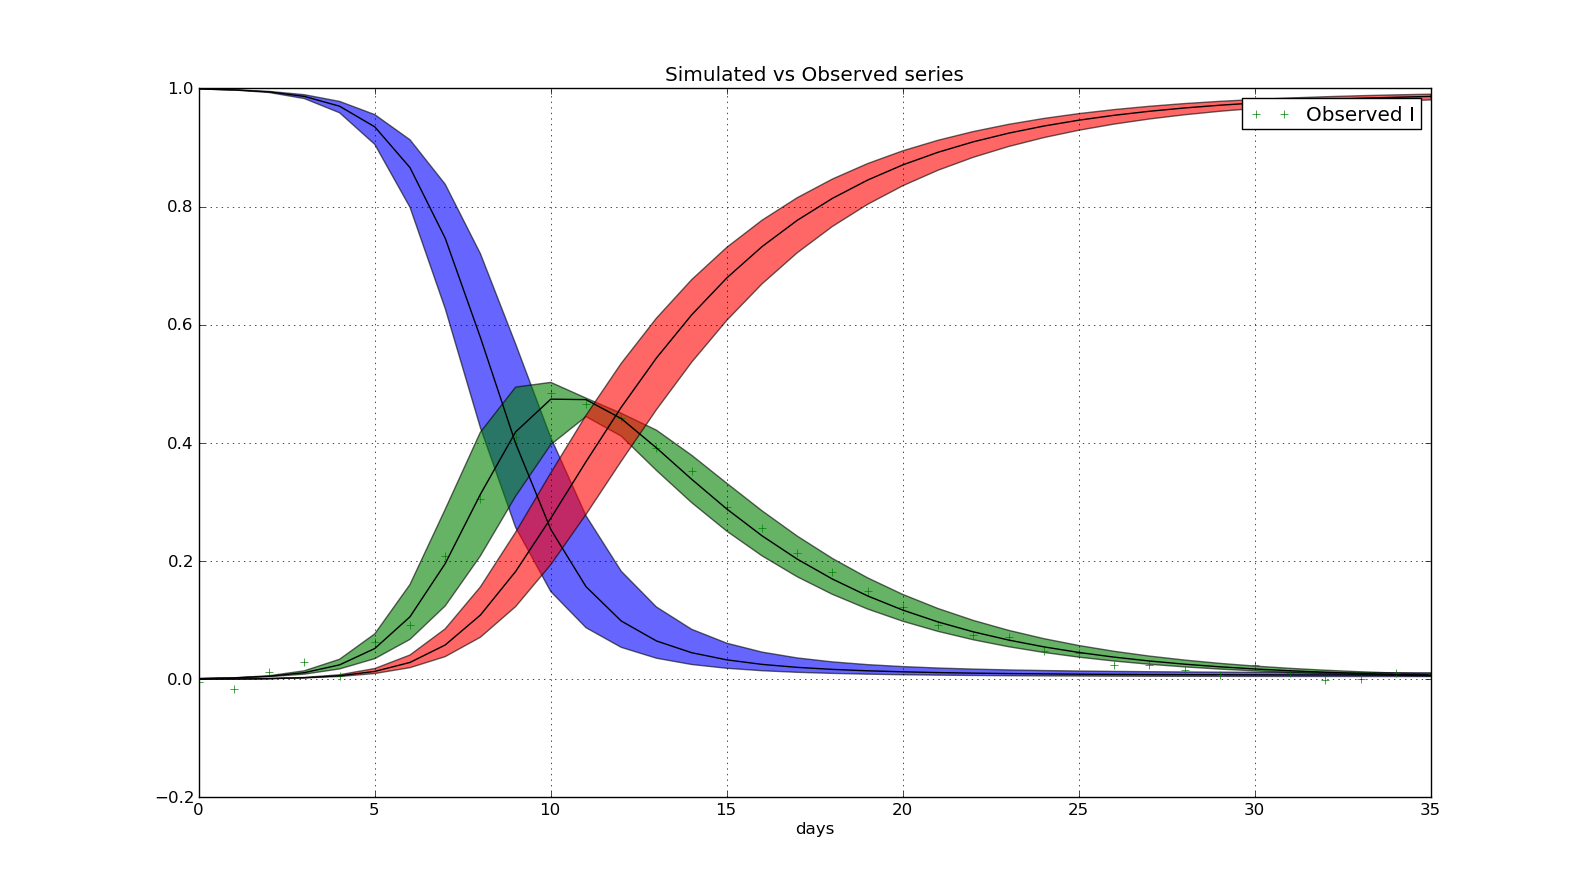
\includegraphics[width=15cm]{fit_series.png}

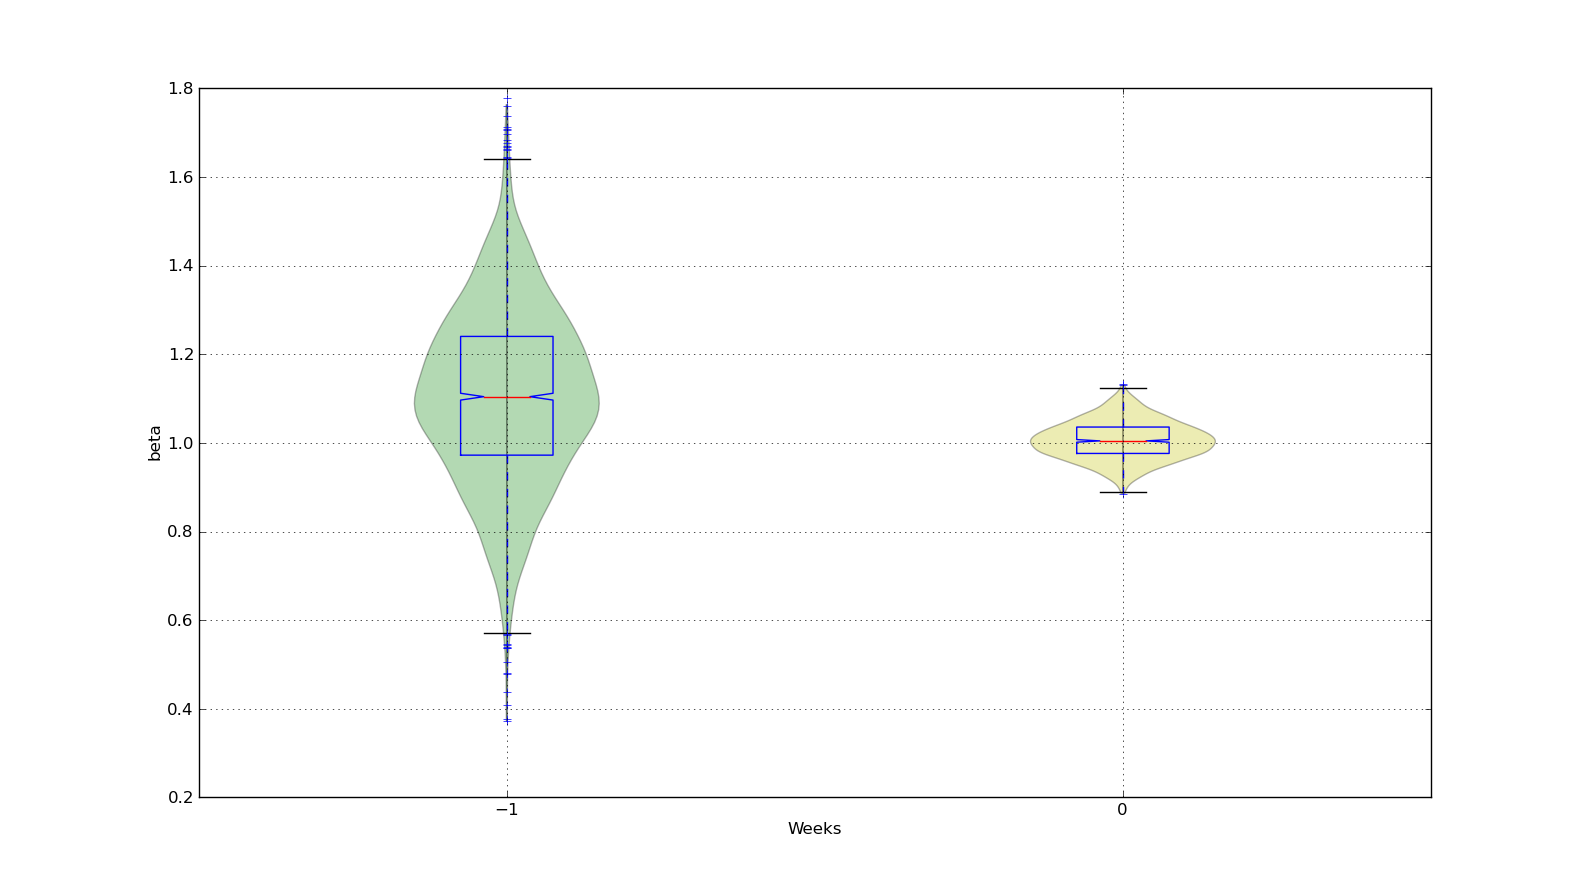
\includegraphics[width=15cm]{fit_par.png}

\resetcurrentobjects
\hypertarget{--doc-sde}{}

\chapter{Stochastic Differential Equations}

The SDE package in BIP, was born out of the need to simulate stochastic model to test the Parameters estimation routines in the Bayes Package. However, it is useful in many general-purpose application since it provides a pure Python implementation of an SDE solver.

Currently it provides a single solving algorithm, the Gillespie SSA. but other algorthms are planned for future releases


\chapter{Indices and tables}
\begin{itemize}
\item {} 
\emph{Index}

\item {} 
\emph{Module Index}

\item {} 
\emph{Search Page}

\end{itemize}


\renewcommand{\indexname}{Module Index}
\printmodindex
\renewcommand{\indexname}{Index}
\printindex
\end{document}
